\subsection{Tabela de Símbolos}
\label{sec:symtab}

Segundo \citeonline{new-dragon-pt}, ``\emph{Tabelas de Símbolos} são
estruturas de dados utilizadas pelos compiladores para conter informações
sobre as construções do programa-fonte''. Essas informações são coletadas
durante as fases de análise (Léxica e Sintática) e utilizadas durante
a fase de geração do programa-objeto (também conhecida como fase de
\emph{síntese}).

As entradas na tabela de símbolos contém informações sobre
identificadores; nome ou seu lexema, posição de memória, seu tipo, entre
outras informações que o implementador julgar necessárias.

As principais operações sobre Tabelas de Símbolos são \emph{inserir},
\emph{consultar} e \emph{remover} uma entrada. Dessa forma, precisamos de uma
estrutura de dados que permita executar essas operações eficientemente.
Foi escolhida a estrutura de \emph{Tabela de Hash Encadeada} para sua
implementação (verificar Seção \ref{sec:hashing}).

Tabelas de símbolos, também, são comumente utilizadas para manter
informações de escopo dos identificadores. Como neste projeto teremos
apenas um escopo global, não discutiremos esse tema, entretanto, mais
referências podem ser encontradas em \citeonline{new-dragon-pt} e
\citeonline{louden97-pt}.


\subsubsection{Hashing (Transformação de Chave)}
\label{sec:hashing}

\emph{Hashing} é um método de pesquisa que utiliza uma função de
transformação da chave de pesquisa para calcular o endereço em que a
entrada será armazenada.

\begin{figure}
	\begin{center}
		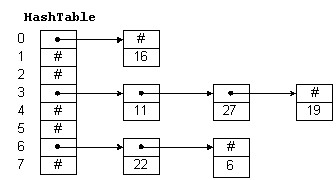
\includegraphics[scale=0.6]{hashtable.png}
	\end{center}
	\caption{Tabela de Hashes}
	\label{fig:hashtable}
\end{figure}

Como podemos observar na Figura \ref{fig:hashtable}, temos as chaves $6, 11,
16, 19, 22, 27$ inseridas na tabela. Também é possível perceber que a
chave com valor $16$ está inserida no endereço $0$ da tabela. Para efetuar
o mapeamento entre as chaves e os endereços é necessário a utilização de
uma função de \emph{hashing} (ou função de \emph{transformação}).

Uma \textbf{função de hashing} deve mapear uma chave, o nome de um
identificador, por exemplo, em inteiros dentro do intervalo $[0..M-1]$ em
que $M$ é o tamanho da tabela. Considerando que as transformações sobre
as chaves são aritméticas, o primeiro passo é transformar as chaves
não-numéricas em números. Para isso, podemos utilizar, por exemplo, o valor
inteiro conforme a \emph{Tabela ASCII} \cite{ziviani}.

\begin{equation} \label{eq:hash}
h(K) = K \text{mod} \, M
\end{equation}

A Equação \ref{eq:hash} demonstra uma das formas de calcular a função
\emph{hash} de uma chave $K$. Nela calculamos o resto da divisão de $K$
pelo tamanho $M$ do arranjo que armazenará a tabela.

\begin{equation} \label{eq:k}
K = \sum_{i=0}^{n-1}\text{chave}[i] \times i
\end{equation}

$K$ é definido conforme a Equação \ref{eq:k}. $i$ é o índice do caractere na
cadeia \emph{chave} e $n$ é o tamanho da cadeia. O produto por $i$ é utilizado
para evitar \emph{hashes} iguais quando tratamos de \emph{anagramas}.

Nesse processo há grande possibilidade de duas chaves possuírem \emph{hashes}
iguais, isto é denominado \emph{colisão} de hashes. Uma das formas possíveis
de resolução de \emph{colisões} é utilizar uma \emph{Lista Encadeada}. Dessa
forma, todas as chaves conflitantes são encadeadas em uma lista linear
\cite{ziviani}. Uma demonstração dessa representação é de dada na Figura
\ref{fig:hashtable}.

Outras formas de resolução de \emph{colisões} e outras implementações de
hashes (como Hashing Perfeito) podem ser encontrados em \citeonline{knuth73} e
\citeonline{ziviani}.

